%
% orthogonalkomplement.tex -- Graphik für den Beweis zum Orthogonalkomplement
%
% (c) 2019 Prof Dr Andreas Müller, Hochschule Rapperswil
%
\documentclass[tikz]{standalone}
\usepackage{amsmath}
\usepackage{times}
\usepackage{txfonts}
\usepackage{pgfplots}
\usepackage{csvsimple}
\usetikzlibrary{arrows,intersections,math}
\begin{document}
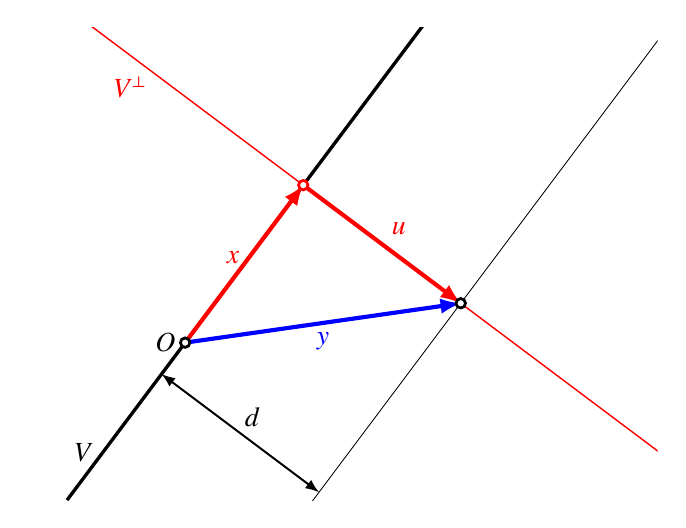
\begin{tikzpicture}[>=latex,scale=1.0]

% add image content here

\def\r{0.06}

\begin{scope}
\clip (-2,-2) rectangle (6,4);

\draw[line width=1.2pt] (-1.5,-2)--(6,8);
\draw[line width=0.5pt,color=red] ({1.5+8},{2-6})--({1.5-8},{2+6});

\def\punkt#1{
	\fill[color=white] #1 circle[radius=\r];
	\draw[line width=1pt] #1 circle[radius=\r];
}

\def\v#1{({#1*3},{#1*4})}
\def\w#1{({2+#1*3},{-1.5+#1*4})}

\coordinate (Y) at (3.5,0.5);
\coordinate (X) at (1.5,2);

\coordinate (C) at ({1.5+0.05*3-2},{2+0.05*4+1.5});

\draw[->,color=blue,line width=1.5pt] (0,0) -- (Y);

\draw[line width=0.3pt] (3.5+6,0.5+8)--(3.5-6,0.5-8);

\node[color=blue] at ({0.5*(1.5+2)},{0.5*(2-1.5)}) [below] {$y$};

\node at (0,0) [left] {$O$};

\draw[->,line width=1.5pt,color=red] (0,0)--(X);
\draw[<-,line width=1.5pt,color=red] (Y)--(X);
\node[color=red] at (2.5,1.25) [above right] {$u$};

\fill[color=white] (X) circle[radius=\r];
\draw[line width=1pt,color=red] (X) circle[radius=\r];

\node[color=red] at \v{0.27} [left] {$x$};
%\node at \v{0.535} [right] {$\bar{x}$};

%\draw[->,line width=0.7pt] (Y)--\v{0.40};
%\draw[->,line width=0.7pt] (Y)--\v{0.65};
%\draw[->,line width=0.7pt] (Y)--(C);
%\draw[->,line width=0.7pt] \v{0.40}--(C);
%\draw[->,line width=0.7pt] \v{0.65}--(C);

\draw[<->,line width=0.7pt] \v{-0.1}--\w{-0.1};

\punkt{(0,0)}

%\punkt{\v{0.40}}
%\punkt{\v{0.65}}
%\punkt{\v{0.525}}
\punkt{({1.5+2},{2-1.5})}
%\punkt{(C)}

%\node at \v{0.40} [left] {$x_m$};
%\node at \v{0.65} [right] {$x_n$};

\node at \v{-0.35} [left] {$V$};

\node[color=red] at ({1.5-2-0.2},{2+1.5}) [below] {$V^{\perp}$};

\node at ({-0.05*3+1},{-0.05*4-0.75}) {$d$};

\end{scope}

\end{tikzpicture}
\end{document}

